248. \begin{figure}[ht!]
\center{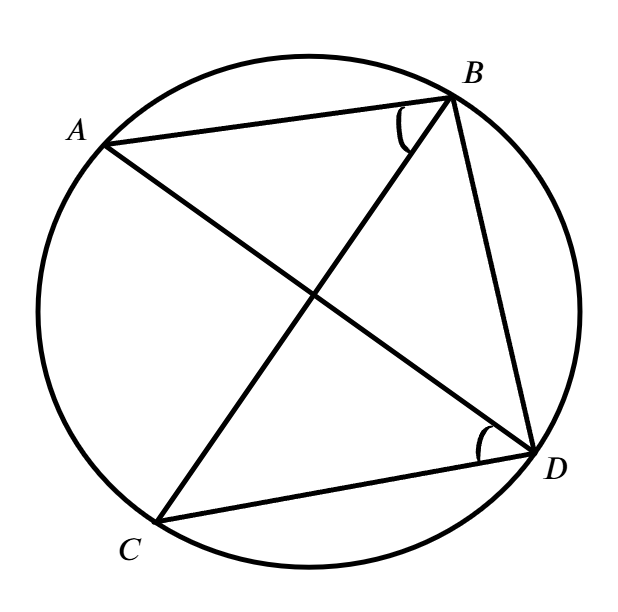
\includegraphics[scale=0.35]{g8-244.png}}
\end{figure}\\
Для того, чтобы равные углы $\angle ADC$ и $\angle CBA$ опирались на одну и ту же дугу $AC,$ точки должны быть расположены в следующем порядке: $A,\ B,\ D,\ C.$ Тогда дуга $AC=2\cdot 52^\circ=104^\circ,$ дуга $AB=2\cdot43^\circ=86^\circ,$ дуга $BDC=360^\circ-104^\circ-86^\circ=170^\circ,$ откуда $\angle BAC=\cfrac{1}{2}\cdot 170^\circ=85^\circ.$\\
